% SIAM Article Template
\documentclass[review,hidelinks,onefignum,onetabnum]{siamart220329}

% Information that is shared between the article and the supplement
% (title and author information, macros, packages, etc.) goes into
% ex_shared.tex. If there is no supplement, this file can be included
% directly.

% Packages and macros go here
\usepackage{lipsum}
\usepackage{amsfonts}
\usepackage{epstopdf}
\usepackage{url}
\usepackage{afterpage}
% \usepackage{algorithmic}
\ifpdf
  \DeclareGraphicsExtensions{.eps,.pdf,.png,.jpg}
\else
  \DeclareGraphicsExtensions{.eps}
\fi

%%%%%%%%%%%%%%%%%%%%%%%%%%%%%%%%%%%%%%%%%%%%%%%%%%%%%%%%%%%%%%%%%
% Paul's commands - note that some had to be commented out

\usepackage[normalem]{ulem}
\usepackage[labelfont=bf, size=small]{caption}
\usepackage[labelformat=empty, size=small]{subcaption}


\usepackage{microtype, fancyhdr,
  siunitx, graphicx, hyperref, epstopdf, tikz, adjustbox, mathtools, float,
  anyfontsize, relsize}
\usepackage{bm, amssymb, amsmath, mathrsfs}
\usepackage{etoolbox}
\usepackage[algo2e, ruled, linesnumbered, resetcount]{algorithm2e}
\SetFuncSty{textsc}
\SetKwProg{Function}{}{:}{}
\SetKwComment{Comment}{$\triangleright$\ }{}


\newcommand{\I}{\mathcal{I}}   % Identity matrix
\newcommand{\E}{\mathbb{E}}    % Expectation
\newcommand{\V}{\mathbb{V}}    % Variance
\newcommand{\Z}{\mathbb{Z}}    % Integers
\newcommand{\Q}{\mathbb{Q}}    % Rational numbers
\newcommand{\R}{\mathbb{R}}    % Real numbers
\newcommand{\C}{\mathbb{C}}    % Complex numbers
\newcommand{\B}{\mathcal{B}}   % Borel set
\newcommand{\X}{\mathcal{X}}   % Italic X
\newcommand{\bO}{\mathcal{O}}  % "big O"
\newcommand{\Hs}{\mathcal{H}}  % Hilbert space
\newcommand{\Sc}{\mathcal{S}}  % Schwartz Class
\newcommand{\Fr}{\mathcal{F}}  % Fourier Transform operator
\newcommand{\Pw}{\mathcal{P}}  % Power set
\newcommand{\Nd}{\mathcal{N}}  % Normal distribution
\newcommand{\Pb}{\mathbb{P}}   % Probability set
\newcommand{\sv}{\, | \,}      % spaced vertical bar
\newcommand{\bt}{\beta}        % beta
\newcommand{\eps}{\varepsilon} % epsilon
\newcommand{\lam}{\lambda}     % lambda
\newcommand{\tht}{\theta}      % theta
\newcommand{\sgm}{\sigma}      % sigma
\newcommand{\omg}{\omega}      % omega
\newcommand{\gam}{\gamma}      % gamma
\newcommand{\bx}{\bm{x}}       % bold x
\newcommand{\by}{\bm{y}}       % bold y
\newcommand{\bv}{\bm{v}}       % bold v
\newcommand{\bu}{\bm{u}}       % bold u
\newcommand{\bz}{\bm{z}}       % bold z
\newcommand{\bw}{\bm{\omega}}  % bold omega
\newcommand{\bmu}{\bm{\mu}}    % bold mu
\newcommand{\bth}{\bm{\theta}} % bold theta
\newcommand{\bet}{\bm{\eta}}   % bold eta
\newcommand{\bS}{\bm{\Sigma}}  % bold Sigma
\newcommand{\bA}{\bm{A}}       % bold A
\newcommand{\syd}{\triangle}     % symmetric difference
\newcommand{\sem}{\setminus}     % set minus
\newcommand{\abs}[1]{\left|#1\right|}      % absolute value
\newcommand{\br}[1]{\overline{#1}}         % bar
\newcommand{\wht}[1]{\widehat{#1}}         % hat
\newcommand{\cvd}{\rightsquigarrow}        % convergence in distribution
\newcommand{\beps}{\bm{\eps}}              % bold epsilon
\newcommand{\pref}[1]{(\ref{#1})}          % ref in parentheses
\newcommand{\ind}[1]{\bm{1}_{\set{#1}}}    % Indicator function
\newcommand{\red}[1]{{\color{red} #1}}     % red text that is robust
\newcommand{\blue}[1]{{\color{blue} #1}}   % blue text that is robust
\newcommand{\dif}[1]{\mathop{}\!\mathrm{d}{#1}}   % d for dx in integral
% norm (\norm[p]{\bx} for p norm)
\newcommand{\norm}[2][]{\left\Vert#2\right\Vert_{#1}} % norm
\newcommand{\shortnorm}[2][]{\Vert#2\Vert_{#1}}       % short norm
\newcommand{\set}[1]{\left\{ #1\right\}}              % set notation
\newcommand{\flr}[1]{{\left\lfloor #1 \right\rfloor}} % floor function
\newcommand{\inp}[1]{\left\langle #1 \right\rangle}   % inner product
\newcommand{\mat}[1]{\begin{bmatrix}#1\end{bmatrix}}  % matrix
\newcommand{\tr}{\mathrm{tr}}
\renewcommand{\epsilon}{\varepsilon}

\DeclareMathOperator*{\Cov}{Cov} 
\DeclareMathOperator*{\Var}{Var}
\DeclareMathOperator*{\argmin}{arg\,min}   % argmin
\DeclareMathOperator*{\argmax}{arg\,max}   % argmax
\DeclareMathOperator*{\logdet}{logdet}     % logdet
\let\Re\relax \DeclareMathOperator*{\Re}{Re} 
\let\Im\relax \DeclareMathOperator*{\Im}{Im}
\newcommand{\range}[2]{#1\hspace*{-0.2em}:\hspace*{-0.2em}#2} % index range
\newcommand{\der}[2]{\frac{d #1}{d #2}} % derivative
\newcommand{\pder}[2]{\frac{\partial #1}{\partial #2}} % partial derivative
\newcommand{\iid}{\mathrel{\overset{\scalebox{0.5}{\text{i.i.d.}}}{\scalebox{1.1}[1]{$\sim$}}}}
% iid

\newtheorem{theorem}{Theorem}
\newtheorem*{theorem*}{Theorem}
\newtheorem{lemma}{Lemma}
\newtheorem*{lemma*}{Lemma}
\newtheorem{corollary}{Corollary}
\newtheorem*{corollary*}{Corollary}
\newtheorem{definition}{Definition}
\newtheorem*{definition*}{Definition}
\newtheorem{proposition}{Proposition}
\newtheorem*{proposition*}{Proposition}
\theoremstyle{remark}
\newtheorem{remark}{Remark}
\newtheorem*{remark*}{Remark}

\numberwithin{equation}{section}

\newcommand{\todocite}{\red{[CITE]}}


\def\spacingset#1{\renewcommand{\baselinestretch}%
{#1}\small\normalsize} \spacingset{1}

\sisetup{exponent-mode=input, retain-zero-exponent=true}

%%%%%%%%%%%%%%%%%%%%%%%%%%%%%%%%%%%%%%%%%%%%%%%%%%%%%%%%%%%%%%%

% Add a serial/Oxford comma by default.
\newcommand{\creflastconjunction}{, and~}

% Used for creating new theorem and remark environments
\newsiamremark{remark}{Remark}
\newsiamremark{hypothesis}{Hypothesis}
\crefname{hypothesis}{Hypothesis}{Hypotheses}
\newsiamthm{claim}{Claim}

% Sets running headers as well as PDF title and authors
\headers{A Nonuniform Fast Hankel Transform}{Paul G. Beckman and Michael O'Neil}

% Title. If the supplement option is on, then "Supplementary Material"
% is automatically inserted before the title.
\title{A Nonuniform Fast Hankel Transform\thanks{Submitted to the editors DATE.
    \funding{P. G. Beckman was partially supported by the Office of Naval
    Research under award \#N00014-21-1-2383 and by the U.S.  Department of
    Energy, Office of Science, Office of Advanced Scientific Computing Research,
    Department of Energy Computational Science Graduate Fellowship under Award
    Number DE-SC0022158. M. O'Neil was partially supported by the Office of
    Naval Research under award \#N00014-21-1-2383.}  } }

% Authors: full names plus addresses.
\author{Paul G. Beckman\thanks{Courant Institute, New York University, New York, NY\\
  (\email{paul.beckman@cims.nyu.edu}, \url{https://cims.nyu.edu/\~pgb8409}).}
\and Michael O'Neil\thanks{Courant Institute, New York University, New York, NY\\
  (\email{oneil@cims.nyu.edu}, \url{https://cims.nyu.edu/\~oneil}).}
}

\usepackage{amsopn}
\DeclareMathOperator{\diag}{diag}

% Optional PDF information
\ifpdf
\hypersetup{
  pdftitle={A Nonuniform Fast  Hankel Transform}
  pdfauthor={P. G. Beckman and M. O'Neil}
}
\fi

% The next statement enables references to information in the
% supplement. See the xr-hyperref package for details.

%\externaldocument[][nocite]{ex_supplement}

% FundRef data to be entered by SIAM
%<funding-group specific-use="FundRef">
%<award-group>
%<funding-source>
%<named-content content-type="funder-name"> 
%</named-content> 
%<named-content content-type="funder-identifier"> 
%</named-content>
%</funding-source>
%<award-id> </award-id>
%</award-group>
%</funding-group>

\begin{document}

\maketitle

% REQUIRED
\begin{abstract}
  In this work we describe a fast algorithm for computing Hankel transforms of
moderate order which combines local and asymptotic expansions with nonuniform
fast Fourier transforms. The resulting algorithm executes in~$\bO (n \log n)$
time, where~$n$ denotes the number of points in both space and frequency.  The
algorithm can be executed to arbitrary precision $\epsilon$, with the order of
the local and asymptotic expansions adjusted automatically according to
analysis. Several numerical examples are provided which demonstrate the speed of
the algorithm in multiple regimes, i.e. varying distributions of points and
varying orders.

\end{abstract}

% REQUIRED
\begin{keywords}
Hankel transform, fast Fourier transform, asymptotic expansion, Bessel function
\end{keywords}

% REQUIRED
\begin{MSCcodes}
XXXX, XXXX, XXXX
\end{MSCcodes}

\section{Introduction} 
The Hankel or Fourier-Bessel transform of order $\nu$ of a function $f : (0,
\infty) \to \C$ is given by
\begin{equation} \label{eq:HT}
    g(\omega) = \int_0^\infty f(r) J_\nu(\omega r) r \dif{r}.
\end{equation}
Discretizing this integral, we obtain the discrete Hankel transform (DHT)
\begin{equation} \label{eq:DHT}
    g_j = \sum_{k=1}^m c_k J_\nu(\omega_j r_k)
\end{equation}
for $j=1, \dots, n$, which can be written equivalently as the matrix-vector
product with $\bm{A} \in \R^{n \times m}$
\begin{equation}
    \bm{g} = \bm{A}\bm{c}, \qquad \bm{A}_{jk} = J_\nu(\omega_j r_k).
\end{equation}
These transforms appear in a wide range of applications including
imaging~\citep{higgins1988hankel, zhao2013fourier}, partial differential
equations~\citep{bisseling1985fast,ali1999generalized}, and
statistics~\cite{lord1954a, genton2002nonparametric}. In many such applications,
a fully nonuniform DHT is desired, as the relevant frequencies $\omega_j$ may
not be equispaced, and the most efficient quadrature rule for discretizing
(\ref{eq:HT}) may have nodes $r_k$ which are also not equispaced.

A number of methods exist in the literature to evaluate (\ref{eq:HT}) or
(\ref{eq:DHT}). These include series expansion methods
\citep{lord1954b,brunol1977fourier,cavanagh1979numerical}, convolutional
approaches \citep{siegman1977quasi, johansen1979fast, mook1983algorithm}, and
projection-slice or Abel transform-based methods
\citep{oppenheim1980computation, hansen1985fast, kapur1995algorithm}.
See~\cite{cree1993algorithms} for a review of many of these early computational
approaches. Unfortunately, these existing methods are either not applicable to
the discrete case (\ref{eq:DHT}), require a particular choice of $\omega_j$ or
$r_k$ due to the constraints of interpolation or quadrature subroutines, or
suffer from low accuracy as a result of intermediate approximations. Therefore,
extending these schemes to compute the fully nonuniform DHT with controllable
accuracy is not straightforward. 

More recently, butterfly algorithms \citep{oneil2010algorithm, li2015butterfly,
pang2020interpolative} were introduced as a broadly applicable methodology for
rapidly computing oscillatory transforms including the nonuniform DHT. However,
these algorithms require a precomputation or factorization stage for each new
set of $\omega_j$ and $r_k$, which can be a bottleneck for applications in which
these evaluation points change with each evaluation. In order to provide a
precomputation-free fast DHT,~\cite{townsend2015fast} uses a combination of
asymptotic expansions and Bessel function identities applicable to equispaced or
perturbed ``quasi-equispaced'' grids, for example $j_{\nu,k} / j_{\nu,n+1}$
where $j_{\nu,k}$ is the $k^{th}$ zero of $J_\nu$.

We describe here a fully nonuniform fast Hankel transform (NUFHT) which
generalizes~\cite{townsend2015fast} in a number of ways. First, we employ an
adaptive partitioning scheme which, for any choice of $r_k$ and $\omega_j$,
subdivides $\bm{A}$ into blocks for which matrix-vector products can be
evaluated efficiently. Second, we use the nonuniform fast Fourier transform
(NUFFT) \citep{dutt1993fast, greengard2004accelerating} to evaluate asymptotic
expansions for nonuniform $r_k$ and $\omega_j$. Finally, we introduce the
low-rank expansion of \cite{wimp1962polynomial} in the local regime where
asymptotic expansions are not applicable. We derive error bounds for this
low-rank expansion, allowing us to choose all approximation parameters
automatically through error analysis which guarantees that the resulting error
is bounded by the user-specified tolerance $\epsilon$. 



\section{Overview of the algorithm} \label{sec:overview}

To more concisely describe our approach, we write the DHT (\ref{eq:DHT}) as the
equivalent matrix-vector product with $\mtx{A} \in \R^{m \times n}$
\begin{equation}
    \vct{g} = \mtx{A}\vct{f}, \qquad \mtx{A}(j,k) = J_\nu(\omega_j r_k).
\end{equation}
The matrix $\mtx{A}$ is in general full rank and possesses complex oscillatory
structure. As a result, no straightforward fast algorithm exists to apply the
full matrix $\mtx{A}$ to a vector. However, we devise an NUFHT by noting that
certain \textit{blocks} $\mtx{A}(j_0:j_1, k_0:k_1)$ are able to be applied to a
vector rapidly using analytical expansions of the underlying Bessel function
$J_\nu$. 

\begin{figure}[!t]
  \centering
  \begin{subfigure}[b]{0.45\textwidth}
    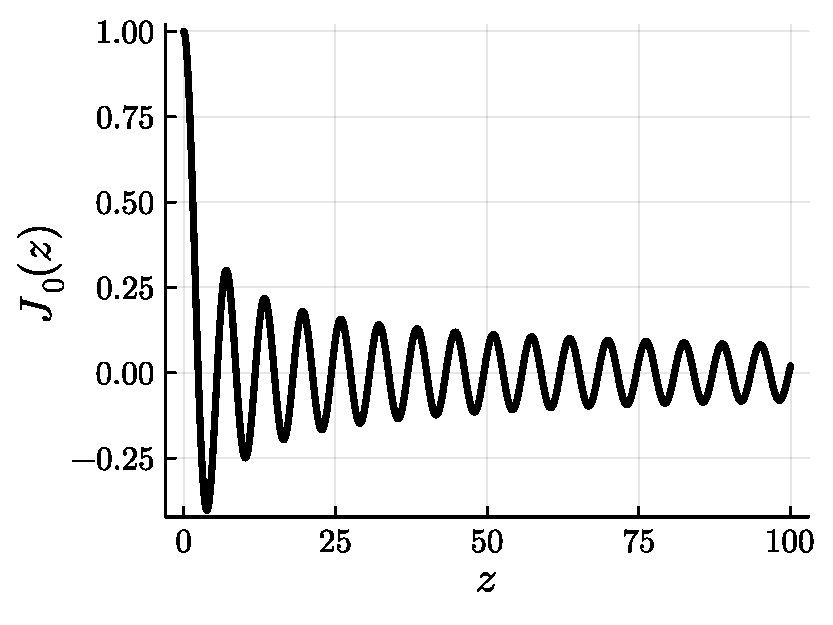
\includegraphics[width=\textwidth]{./figures/bessel_function.pdf}
  \end{subfigure}
  \begin{subfigure}[b]{0.45\textwidth}
    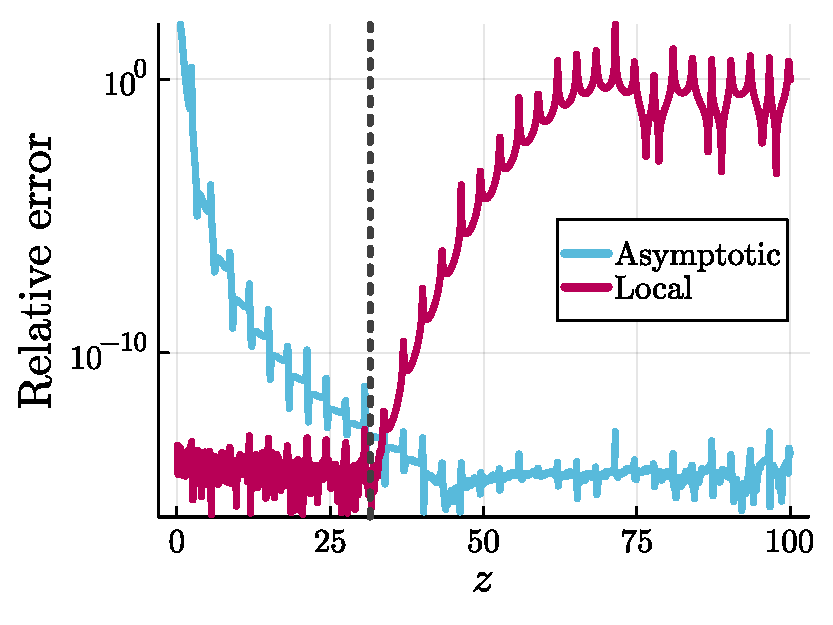
\includegraphics[width=\textwidth]{./figures/pointwise_errors.pdf}
  \end{subfigure}
  \caption{Bessel function $J_0(z)$ and pointwise relative error in
  approximating $J_0(z)$ using local and asymptotic expansions. Dotted vertical
  line shows crossover point where both expansions are accurate to $\epsilon =
  10^{-12}$.}
  \label{fig:two-expansions}
\end{figure}

When the argument $\omega_j r_k$ is small, $J_\nu$ is smooth and essentially
non-oscillatory, and we use a closed-form local expansion which approximates
$J_\nu$ in terms of Chebyshev polynomials, yielding a low-rank approximation to
the block $\mtx{A}(j_0:j_1, k_0:k_1)$ that can be applied to a vector in linear
time. When the argument $\omega_j r_k$ is large, we use a classical asymptotic
expansion which expresses $J_\nu$ as a sum of a small number of decaying
sinusoids, and can therefore be applied to a vector in quasilinear time using
the NUFFT. Figure~\ref{fig:two-expansions} shows the oscillatory behavior of
$J_0$, as well as the accuracy of these local and asymptotic expansions.

By analyzing the error in these two expansions, we can choose a threshold $z$
such that an $L$-term local expansion and an $M$-term asymptotic expansion are
both guaranteed to be accurate to the desired accuracy $\epsilon$ in the regions
$\omega_j r_k \leq z$ and $\omega_j r_k > z$ respectively. Next, we adaptively
subdivide $\mtx{A}$ into disjoint blocks so that either $\omega_j r_k \leq z$ or
$\omega_j r_k > z$ for all $\omega_j$ and all $r_k$ in each block. This leaves
only a few small blocks with $\omega_j r_k \approx z$ whose entries are directly
computed. Finally, we apply each of these disjoint blocks of $\mtx{A}$ to
$\vct{f}$ using the corresponding fast method. Figure~\ref{fig:subdivide} shows
an Hankel transform matrix $\mtx{A}$ divided into local and asymptotic entries
along the curve $\omega r = z$, as well as the corresponding adaptive
subdivision of the matrix into blocks which can be rapidly applied.

\begin{figure}
  \centering
  \newcommand\twa{0.29cm} \newcommand\tw{0.43cm}
  \begin{subfigure}[b]{0.28\textwidth}
    \begin{tikzpicture}
        \draw (0, 0) node[inner sep=0] {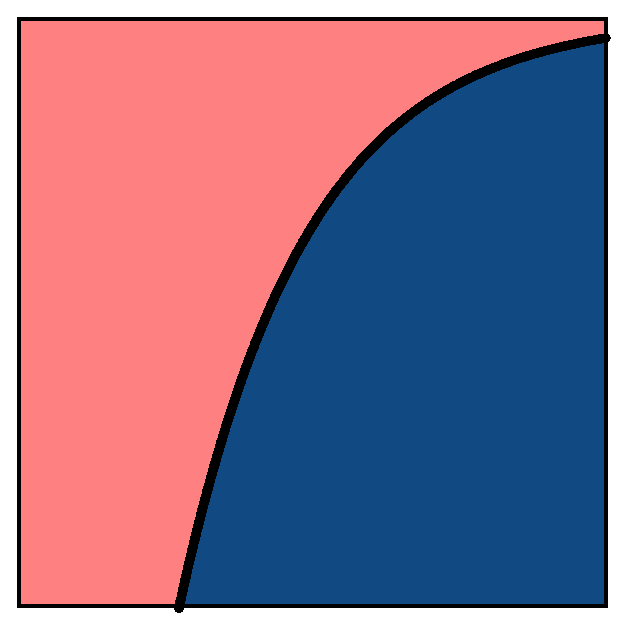
\includegraphics[width=0.75\textwidth,
        trim={\twa, \twa, \twa, \twa}, clip]{./figures/splitting.pdf}}; \draw
        (-0.8, 0.8) node {\small \textbf{Local}}; \draw (0.3, -0.7) node {\small
        \textbf{Asymptotic}}; \draw (0, 1.6) node {\small $r_1 \ \; < \ \dots \
        < \ \; r_n$}; \draw (-1.7, 0) node[align=center] {\small $\omega_1$
        \\[3pt] $\wedge$ \\[3pt] $\vdots$ \\[3pt] $\wedge$ \\[3pt] $\omega_m$};
    \end{tikzpicture}
    \caption{}
  \end{subfigure}
  \hspace*{0.0\textwidth}
  \begin{subfigure}[b]{0.21\textwidth}
    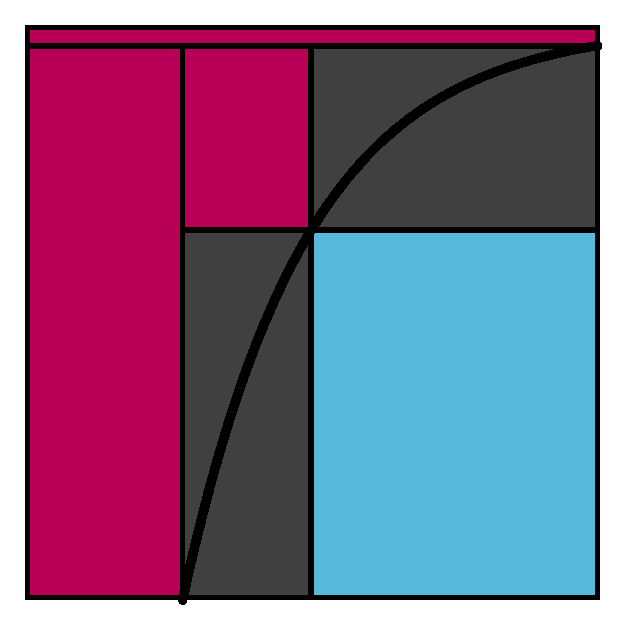
\includegraphics[width=\textwidth, trim={\tw, \tw, \tw, \tw}, clip]{./figures/splitting_lvl1.pdf}
    \caption{Level 1}
  \end{subfigure}
  \hfill
  \begin{subfigure}[b]{0.21\textwidth}
    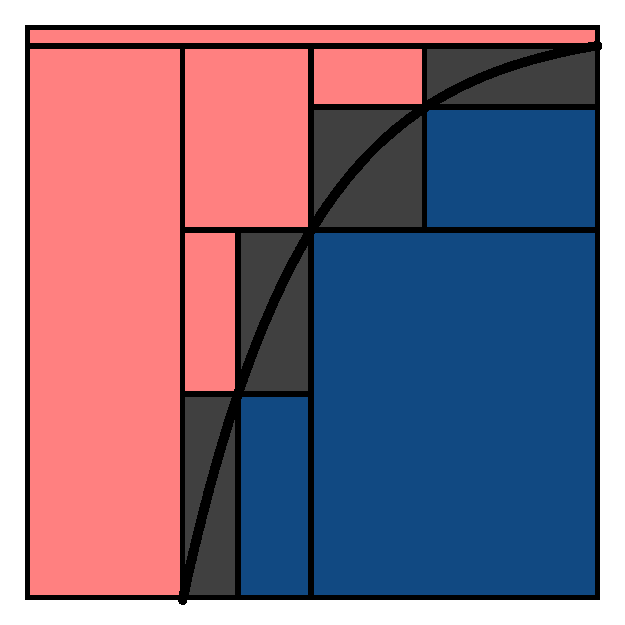
\includegraphics[width=\textwidth, trim={\tw, \tw, \tw, \tw}, clip]{./figures/splitting_lvl2.pdf}
    \caption{Level 2}
  \end{subfigure}
  \hfill
  \begin{subfigure}[b]{0.21\textwidth}
    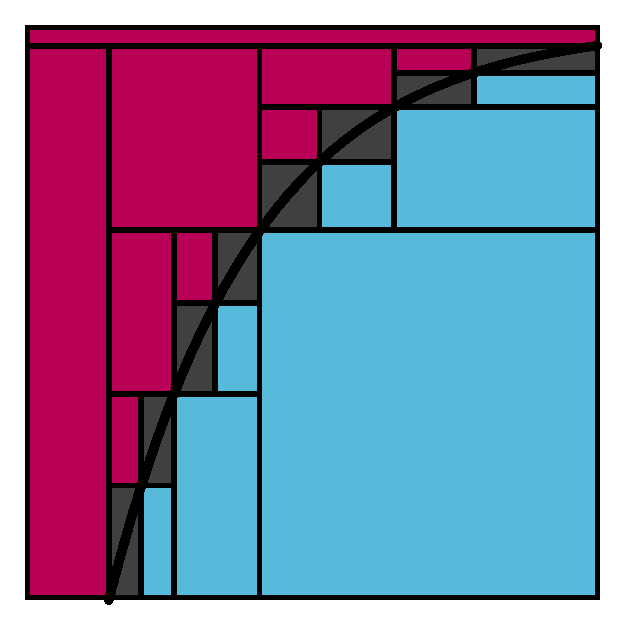
\includegraphics[width=\textwidth, trim={\tw, \tw, \tw, \tw}, clip]{./figures/splitting_lvl3.pdf}
    \caption{Level 3}
  \end{subfigure}
  \caption{Splitting of Hankel transform matrix $\mtx{A}$ along the curve
  $\omega r = z$ into local and asymptotic regions. Adaptive subdivision of
  $\mtx{A}$ into corresponding local (red), asymptotic (blue), and mixed (gray)
  sub-blocks at various levels.}
  \label{fig:subdivide}
\end{figure}

\section{Bessel function approximations} \label{sec:approx}
We now describe local and asymptotic expansions of the Bessel function
$J_\nu(\omega r)$, and provide error analysis by which one can select the number
of terms needed in each expansion to assure $\epsilon$ accuracy in both regimes.

\subsection{The Wimp expansion}\label{sec:local}

Near the origin, $J_\nu(z)$ is a smooth and essentially non-oscillatory function
of $z$. As a result, $J_\nu(xy)$ is a numerically low-rank function of all
sufficiently small inputs $x$ and $y$. Fortuitously, one such low-rank expansion
--- which we refer to as the \textit{Wimp expansion} --- is available in closed
form for integer $\nu$~\cite{wimp1962polynomial}. In the case that $\nu$ is
even, we have
\begin{equation}
    \begin{aligned}
        J_\nu(xy) 
        &= \sum_{\ell=0}^\infty C_\ell(x) T_{2\ell}(y) \\
        C_\ell(x) 
        &= \delta_\ell J_{\frac{\nu}{2} + \ell}(x) \, J_{\frac{\nu}{2} - \ell}(x) \\
        \delta_\ell 
        &= \begin{cases}
            1 & \ell=0 \\
            2 & \text{otherwise}
        \end{cases}
    \end{aligned}
\end{equation}
for all $\abs{y} \leq 1$. A similar expansion exists for $\nu$ odd.

In order to employ the Wimp expansion to compute local terms within the Hankel
transform, we must determine the number of terms $L$ needed to construct an
$\epsilon$-accurate approximation to $J_\nu(\omega r)$ on a given rectangle
$(\omega, r) \in [0, \Omega] \times [0, R]$. The following lemma provides a
bound on the induced truncation error in the Wimp expansion as a function of the
order $\nu$, the space-frequency product $\Omega R$, and the number of retained
terms $L$.

\begin{lemma} \label{lem:wimp} Truncating the Wimp expansion after $L$ terms
    gives
    \begin{align}
        \abs{J_\nu(\omega r) - \sum_{\ell=0}^L C_\ell(\omega R) T_{2\ell}\left( \frac{r}{R} \right)} 
        \leq \frac{2\exp\left\{ \frac{\nu}{2}(\beta - \gamma) + (L+1)(\beta + \gamma) \right\}}{1 - e^{\beta + \gamma}}
    \end{align}
    for all $\omega \in [0, \Omega], r \in [0, R]$, where
    \begin{align}
        \psi(p) &:= \log p + \sqrt{1 - p^2} - \log\left( 1 + \sqrt{1 - p^2} \right) \\
        \beta &:= \psi\left( \frac{\Omega R}{2L + 2 + \nu} \right) \\
        \gamma &:= \begin{cases}
            \psi\left( \frac{\Omega R}{2L + 2 - \nu} \right) & L + 1 \geq \frac{\nu}{2} \\
            0 & \textnormal{otherwise}
        \end{cases}
    \end{align}
\end{lemma}
\begin{proof}
    For $\nu$ even, the truncation error after $L$ terms is bounded by
    \begin{align}
        \abs{\sum_{\ell=L+1}^\infty C_\ell(\omega R) T_{2\ell}\left( \frac{r}{R} \right)}
        &\leq 2\sum_{\ell=L+1}^\infty \abs{J_{\frac{\nu}{2} + \ell}\left(\frac{\omega R}{2}\right)} \abs{J_{\frac{\nu}{2} - \ell}\left(\frac{\omega R}{2}\right)}.
    \end{align}
    Define $p_\ell(\omega) := \omega R / (\nu + 2\ell)$. Then by Siegel's bound
    \cite[10.14.5]{olver2010nist} we have
    \begin{align}
        \abs{J_{\frac{\nu}{2} + \ell}\left(\frac{\omega R}{2}\right)}
        &= \abs{J_{\frac{\nu}{2} + \ell}\bigg(\Big(\frac{\nu}{2} + \ell\Big) p_\ell(\omega)\bigg)} \\
        &\leq \exp\left\{ \Big(\frac{\nu}{2} + \ell\Big) \psi\big(p_\ell(\omega)\big)\right\} \\
        &\leq \exp\left\{ \Big(\frac{\nu}{2} + \ell\Big) \beta \right\},
    \end{align}
    where the last inequality follows from the fact that $\psi$ is an increasing
    function on $(0,1)$, and thus $\psi\big(p_\ell(\omega)\big) \leq \beta < 0$
    for all $\ell \geq L+1$ and all $\omega \in [0, \Omega]$. 
    
    If $L+1 \geq \frac{\nu}{2}$, we define $q_\ell(\omega) := \omega R / (2\ell
    - \nu)$ and apply Siegel's bound again to obtain
    \begin{align}
        \abs{J_{\frac{\nu}{2} - \ell}\left(\frac{\omega R}{2}\right)}
        &= \abs{J_{\ell - \frac{\nu}{2}}\bigg(\Big(\ell - \frac{\nu}{2}\Big) q_\ell(\omega)\bigg)} 
        \leq \exp\left\{ \Big(\ell - \frac{\nu}{2}\Big) \gamma \right\}.
    \end{align}
    If $L+1 < \frac{\nu}{2}$, Siegel's bound does not apply and we use instead
    the simple bound $\abs{J_{\frac{\nu}{2} - \ell}\left(\frac{\omega
    R}{2}\right)} \leq 1$, which is equivalent to taking $\gamma = 0$. 

    All that remains is to apply a geometric series argument
    \begin{align}
        \abs{J_\nu(\omega r) - \sum_{\ell=0}^L C_\ell(\omega R) T_{2\ell}\left( \frac{r}{R} \right)}
        &\leq 2\sum_{\ell=L+1}^\infty \exp\left\{ \Big(\frac{\nu}{2} + \ell\Big) \beta + \Big(\ell - \frac{\nu}{2}\Big) \gamma \right\} \\
        &= 2\exp\left\{\frac{\nu}{2}(\beta - \gamma)\right\} \sum_{\ell=L+1}^\infty \left( e^{\beta + \gamma} \right)^\ell \\
        &= \frac{2\exp\left\{ \frac{\nu}{2}(\beta - \gamma) + (L+1)(\beta + \gamma) \right\}}{1 - e^{\beta + \gamma}}
    \end{align}
    A similar calculation can be carried out for $\nu$ odd.
\end{proof}

Lemma \ref{lem:wimp} is rather opaque regarding the impact of the various
parameters on the error because we have not utilized any simplifying bounds on
the function $\psi$. However, it takes into account the decay in both
$J_{\frac{\nu}{2}+\ell}$ \textit{and} $J_{\frac{\nu}{2}-\ell}$, thus remaining
relatively tight for small $\nu$. It is therefore well-suited to our purposes,
because given $z, L > 0$, it gives a bound on the pointwise error in
approximating any block of the matrix $J_\nu(\omega_j r_k)$ for which $\omega r
\leq z$ using the $L$-term Wimp expansion. 

This expansion is highly beneficial from a computational perspective, as it
yields an analytical rank-$L$ approximation to any block of $\bm{A}$ for which
$\omega_j r_k$ is sufficiently small
\begin{equation}
    \mtx{A}(j_0:j_1, k_0:k_1) \vct{f}(k_0:k_1)
    \approx \mtx{C}\mtx{T}^\top \vct{f}(k_0:k_1)
\end{equation}
where $\mtx{C} \in \R^{(j_1-j_0+1) \times L}$ and $\mtx{T} \in \R^{(k_1-k_0+1)
\times L}$ with entries $\mtx{C}(j,\ell) = C_{\ell-1}(\omega_j r_{k_1})$ and
$\mtx{T}(k,\ell) = T_{2\ell-2}\big(\frac{r_k}{r_{k_1}}\big)$. For a block of
$\mtx{A}$ of size $m_b \times n_b$, the low-rank approximation given by the Wimp
expansion can be applied to a vector in $\bO\big(L(m_b + n_b)\big)$ time by
first applying $\bm{T}^\top$ then applying $\bm{C}$.

\subsection{Hankel's expansion}
\label{sec:asymptotic}

Away from the origin, $J_\nu(z)$ exhibits essentially sinusoidal oscillation
with period $2\pi$. This statement is made precise by Hankel's asymptotic
expansion, which states that for $z \to \infty$
\begin{align} \label{eq:asymptotic-expansion}
    J_\nu(x)
    \sim \sqrt{\frac{2}{\pi x}} \left( 
        \cos\left(x + \phi\right) \sum_{\ell=0}^{\infty} \frac{(-1)^\ell a_{2\ell}(\nu)}{x^{2\ell}}
        - \sin\left(x + \phi\right) \sum_{\ell=0}^{\infty} \frac{(-1)^\ell a_{2\ell+1}(\nu)}{x^{2\ell+1}}
        \right)
\end{align}
where $\phi := - \frac{(2\nu+1)\pi}{4}$ and 
\begin{align}
    a_\ell(\nu) := \frac{(4\nu^2 - 1)(4\nu^2 - 3)\dots(4\nu^2 - (2\ell-1)^2)}{\ell! 8^\ell}.
\end{align}
Rearranging this expansion, we obtain an expansion which can be evaluated using
two NUFFTs and diagonal scalings, and whose error is bounded by the size of the
first neglected terms \todocite
\begin{align}
    & \Bigg| J_\nu(\omega r)
    - \sqrt{\frac{2}{\pi}} \sum_{\ell=0}^{M-1} 
        \frac{(-1)^\ell a_{2\ell}(\nu)}{\omega^{2\ell + \frac{1}{2}}} \Re\left( \frac{e^{i\phi}}{r^{2\ell+\frac{1}{2}}} e^{i\omega r}\right)
        - \frac{(-1)^\ell a_{2\ell+1}(\nu)}{\omega^{2\ell+\frac{3}{2}}} \Im\left(\frac{e^{i\phi}}{r^{2\ell+\frac{3}{2}}} e^{i\omega r} \right)
        \Bigg| \\
        &\hspace*{0.1\textwidth} \leq \sqrt{\frac{2}{\pi}} \left( \frac{\abs{a_{2M}(\nu)}}{(\omega r)^{2M+\frac{1}{2}}} + \frac{\abs{a_{2M+1}(\nu)}}{(\omega r)^{2M+\frac{3}{2}}} \right)
\end{align}

The computational advantage of this expansion is that the $2M$-term asymptotic
expansion of any block of $\bm{A}$ can be rapidly applied to a vector using $2M$
Type-III NUFFTs
\begin{align}
    \mtx{A}(j_0:j_1, k_0:k_1) \vct{f}(k_0:k_1) \hspace*{0.2\textwidth}& \\
    \approx \sqrt{\frac{2}{\pi}} \sum_{\ell=0}^{M-1} (-1)^\ell \Bigg[ 
        a_{2\ell}(\nu) \mtx{D}_\omega^{-2\ell-\frac{1}{2}} &\Re\Big(e^{i\phi} \mtx{F} \mtx{D}_r^{-2\ell-\frac{1}{2}} \vct{f}(k_0:k_1)\Big) \\
        - a_{2\ell+1}(\nu) \mtx{D}_\omega^{-2\ell-\frac{3}{2}} &\Im\Big(e^{i\phi} \mtx{F} \mtx{D}_r^{-2\ell-\frac{3}{2}} \vct{f}(k_0:k_1)\Big) 
    \Bigg]
\end{align}
where $\mtx{F} \in \C^{(j_1 - j_0 + 1) \times (k_1 - k_0 + 1)}$ is the Type-III
nonuniform DFT matrix corresponding to frequencies $\omega_{j_0}, \dots,
\omega_{j_1}$ and points $r_{k_0}, \dots, r_{k_1}$, and the diagonal scaling
matrices are given by $\mtx{D}_\omega :=
\diag(\omega_{j_0},\dots,\omega_{j_1})$, and $\mtx{D}_r :=
\diag(r_{k_0},\dots,r_{k_1})$.

\subsection{Determining order of expansions and crossover point}
\label{sec:cutoff}

With these error bounds in hand, we precompute the following tables for
tolerances $\epsilon = 10^{-4}, \dots, \allowbreak 10^{-15}$, orders $\nu = 1,
\dots, 100$, and number of asymptotic expansion terms $M = 1, \dots, 20$:
\begin{itemize}
    \item $z_{\nu, \epsilon}^M$ such that $M$-term Hankel expansion of
    $J_\nu(\omega r)$ is $\epsilon$-accurate $\forall \ \omega r > z_{\nu,
    \epsilon}^M$
    \item $L_{\nu, \epsilon}^M$ such that $L_{\nu, \epsilon}^M$-term Wimp
    expansion of $J_\nu(\omega r)$ is $\epsilon$-accurate $\forall \ \omega r
    \leq z_{\nu, \epsilon}^M$
\end{itemize}
Therefore, for any order $\nu$ we can look up a pair of complementary local and
asymptotic expansions with error everywhere bounded by the requested tolerance
$\epsilon$. The only remaining free parameter is the number of asymptotic terms
$M$. This parameter is selected heuristically in our implementation as 
\begin{align} \label{eq:num-asy-terms}
    M = \min\left(\flr{1 + \frac{\nu}{5} - \frac{\log_{10}(\epsilon)}{4}}, 20\right)
\end{align}
according to numerical experiments which maximize speed by balancing the cost of
the local, asymptotic, and direct evaluations.



%%% Local Variables: %% mode: latex %% TeX-master: "../main" %% End:


\section{The Nonuniform Fast Hankel Transform} \label{sec:methods}

We now describe our NUFHT algorithm in detail, emphasizing the process by which
$\mtx{A}$ is adaptively subdivided into blocks using the results of the above
error analysis.

\subsection{Subdividing the matrix into blocks by expansion}

Having established error bounds which allow us to automatically select the
number of asymptotic terms $M$, local terms $L$, and crossover point $z$ given a
tolerance $\epsilon$ and order $\nu$, we subdivide the matrix $\mtx{A}$ into
three sets of blocks, each of which can be efficiently applied to a vector as
described above:
\begin{itemize}
    \item Local blocks $\mathscr{L} = \big\{ (j_0:j_1, k_0:k_1) \ | \ \omega_j
    r_k \leq z \ \forall \ j_0 \leq j \leq j_1, \ k_0 \leq k \leq k_1 \big\}$
    \item Asymptotic blocks $\mathscr{A} = \big\{ (j_0:j_1, k_0:k_1) \ | \
    \omega_j r_k > z \ \forall \ j_0 \leq j \leq j_1, \ k_0 \leq k \leq k_1
    \big\}$
    \item Direct blocks $\mathscr{D}$ which are small enough that no fast
    expansion is needed
\end{itemize}

In order to determine a subdivision of $\mtx{A}$ into blocks of these three
types, we initialize a set of \textit{mixed} blocks $\mathscr{M} = \{(1:m,
1:n)\}$, each of which contains a mix of local and asymptotic entries. We then
chose an index pair $(j,k)$ such that $\omega_j r_k \approx z$. This index
subdivides the block into four new sub-blocks with $(j,k)$ at the center, so
that the upper left block can be applied using the local expansion and is
appended to $\mathscr{L}$, the lower right block using the asymptotic expansion
and is appended to $\mathscr{A}$. 

The remaining lower left and upper right blocks each still contain a mix of
local and asymptotic entries. If they are of sufficiently small size $m_b \times
n_b$ with $m_b n_b < \texttt{min\_size}$, they can be evaluated directly and are
appended to $\mathscr{D}$. Otherwise they are appended back to $\mathscr{M}$,
and we continue the subdivision process recursively. 

This method yields a valid partition for any choice of $(j,k)$, but for
efficiency these indices are chosen to maximize the number of matrix entries
which can be applied using a fast expansion, i.e. the sizes of the upper left
and lower right blocks. This is done by solving the following constrained
optimization problem
\begin{align}
    (j,k) 
    &\ = \textsc{SplitIndices}(r_1,\dots,r_n, \omega_1,\dots,\omega_m, z) \\
    &:= \left\{
        \begin{array}{r@{\quad } l}
        \displaystyle\argmax_{j,k\in\Z} & (j-j_0)(k_1-k) + (j_1-j)(k-k_0)   \\
        \text{subject to} & j_0 \leq j \leq j_1 \\ 
        & k_0 \leq k \leq k_1 \\ 
        & \omega_j r_k \leq z
        \end{array}
    \right. \label{eq:subdiv-optim}
\end{align}
This problem can be solved exactly in $\bO(j_1-j_0 + k_1-k_0)$ time. However,
computing the exact optimal splitting indices for every box gives a negligible
speedup to the overarching Hankel transform compared to a simpler, quasi-optimal
scheme. In practice it is sufficient to choose a small number of equispaced
indices $j \in j_0:j_1$, compute the corresponding $k = \argmax \{k \ | \ r_k
\leq \frac{z}{\omega_j}\}$ for each $j$, and choose $(j,k)$ as the pair which
minimizes the objective function of (\ref{eq:subdiv-optim}) among this small
collection.

\begin{algorithm2e}[t]
    \caption{Block subdivision of Hankel transform
    matrix}\label{alg:subdivision}
    \SetKwFunction{Subdivide}{Subdivide}
\Function{\Subdivide{$\bm{r}, \bm{\omega}, z, \texttt{\upshape min\_size}$}}{
    $\mathscr{L} = \mathscr{A} = \mathscr{D} = \emptyset$ \\
    $\mathscr{M} = \{(1:m, 1:n)\}$ \\
    \While{$\mathscr{M} \neq \emptyset$}{
        Pop an element $(j_0 : j_1, k_0 : k_1)$ from $\mathscr{M}$ \\
        $(j,k) = \textsc{SplitIndices}(r_{j_0},\dots,r_{j_1}, \omega_{k_0},\dots,\omega_{k_1}, z)$ \\
        Append $(j_0:j, k_0:k)$ to $\mathscr{L}$ \\
        Append $(j+1:j_1, k+1:k_1)$ to $\mathscr{A}$ \\
        Append $(j_0:j, k+1:k_1)$ to $\mathscr{M}$ \textbf{if} $(j - j_0 + 1)(k_1 - k) > \texttt{\upshape min\_size}$ \textbf{else} $\mathscr{D}$ \\
        Append $(j+1:j_1, k_0:k)$ to $\mathscr{M}$ \textbf{if} $(j_1 - j)(k_1 - k + 1) > \texttt{\upshape min\_size}$ \textbf{else} $\mathscr{D}$
    }
    \Return{$(\mathscr{L}, \mathscr{A}, \mathscr{D})$}
}
\end{algorithm2e}

\begin{algorithm2e}[t]
    \caption{Nonuniform fast Hankel transform}\label{alg:nufht}
    \SetKwFunction{NUFHT}{NUFHT}
\Function{\NUFHT{$\nu, \epsilon, \bm{r}, \bm{c}, \bm{\omega}$}}{
    $\bm{g} = \bm{0}$ \\
    Choose $M$ using (\ref{eq:num-asy-terms}) \\
    Look up $L = L_{\nu,\epsilon}^{M}$ and $z = z_{\nu,\epsilon}^{M}$ from pre-computed tables \\
    Choose \texttt{\upshape min\_size} from numerical experiments (e.g. default 1024)
    $(\mathscr{L}, \mathscr{A}, \mathscr{D}) = \textsc{Subdivide}(r_1,\dots,r_n, \omega_1,\dots,\omega_m, z, \texttt{\upshape min\_size})$ \\
    \For{$\mathscr{B} \in (\mathscr{L}, \mathscr{A}, \mathscr{D})$}{
        \For{$(j_0:j_1, k_0:k_1) \in \mathscr{B}$}{
            $\bm{g}(j_0:j_1) \pluseq \bm{A}(j_0:j_1, k_0:k_1) \bm{c}(k_0:k_1)$ using corresponding expansion \\
        }
    }
    \Return{$\bm{g}$}
}
\end{algorithm2e}

\subsection{Complexity analysis}

We now analyze the computational complexity of the proposed approach. In order
to do so, we must first comment on the complexity of the NUFFT, which is an
important subroutine in our method. Most analysis-based NUFFT codes ---
including the \texttt{FINUFFT} library \cite{barnett2019parallel} which we use
in our NUFHT implementation --- consist of three steps. First, delta masses
centered at each non-uniform point are convolved with a \textit{spreading
function} which smears them onto a fine $N$-point uniform grid. Then, a standard
equispaced FFT is computed on the fine grid. Finally, a diagonal de-convolution
with the Fourier transform of the spreading function is applied to reverse the
effect of the original smearing. For a more complete description of this NUFFT
method, see \cite{dutt1993fast,greengard2004accelerating,barnett2019parallel}.
For $n$ points $r_k$ and $m$ frequencies $\omega_j$, spreading of each input
point is $\bO(n)$, the FFT on the fine grid is $\bO(N\log N)$, and the
deconvolution of each output frequency is $\bO(m)$. For the Type-III NUFFT, the
size $N$ of the fine grid typically scales linearly with the space-frequency
product $p := (\omega_m - \omega_1)(r_n - r_1)$ \cite{barnett2019parallel,
greengard2004accelerating}. Therefore the total cost of the NUFFT is $\bO(n + m
+ p\log p)$. Applying this fact in each asymptotic block in the Hankel transform
matrix, and adding the cost of applying local and direct blocks, we can now
analyze the complexity of the entire NUFHT method.

\begin{theorem} \label{thm:complexity} Take $\omega_1 < \dots < \omega_m \in
    [0,\infty)$ and $r_1 < \dots < r_n \in [0,\infty)$ and define the
    space-frequency product $p := (\omega_m - \omega_1)(r_n - r_1)$. Then the
    complexity of computing the NUFHT of order $\nu$ to tolerance $\epsilon$
    using Algorithm \ref{alg:nufht} is 
    $$\bO\Big((L + M)(m + n) \log \min(n,m) + Mp\log p\Big)$$ where $L$ and $M$
    are the number of local and asymptotic terms respectively chosen according
    to $\nu$ and $\epsilon$.
\end{theorem}

\begin{proof}
    Take $z = z_{\nu, \epsilon}^M$. If $\omega_j r_k \leq z$ for all
    $j=1,\dots,n$ and $k=1,\dots,m$ then only the $L$-term low-rank local
    expansion is used, which can be applied in $\bO(L(m + n))$ time. If instead
    $\omega_j r_k > z$ everywhere, then only the $M$-term asymptotic expansion
    is used, which can be applied using the Type-III NUFFT in $\bO(M(m + n +
    p\log p))$ complexity.

    Otherwise consider the case where $\mtx{A}$ contains both local and
    asymptotic entries. First, note that the number of levels
    $N_{\text{level}}$ scales like $\bO(\log\min(n,m))$. The cost of determining the splitting indices $(j,k)$ for each box $\mtx{A}(j_0:j_1,k_0:k_1)$ is $\bO(j_1-j_0+k_1-k_0)$, and thus the total cost of subdivision at each level is $\bO(m+n)$. Therefore the total cost of subdividing $\mtx{A}$ is $\bO((m+n)\log\min(n,m))$.
    
    Now without loss of generality assume $\omega_1 \leq
    \frac{z}{r_n} < \omega_2$ and $r_1 \leq \frac{z}{\omega_m} < r_2$, because
    otherwise we have blocks which can be evaluated using a single expansion as
    described above without affecting the complexity. After step $\ell$ of subdividing every mixed block, we obtain $2^{\ell}$ new
    mixed blocks, $2^{\ell-1}$ new local blocks, and $2^{\ell-1}$ new asymptotic
    blocks. Let the local blocks be of size $m_{\ell,b}^{(\text{loc})} \times
    n_{\ell,b}^{(\text{loc})}$ for $b = 1,\dots,2^{\ell-1}$. Then
    $\sum_{b=1}^{2^{\ell-1}} m_{\ell,b}^{(\text{loc})} \leq m$ and
    $\sum_{b=1}^{2^{\ell-1}} n_{\ell,b}^{(\text{loc})} \leq n$. An analogous
    fact holds for the asymptotic blocks.
    
    Therefore, the total cost of local evaluation is 
    \begin{align}
        \sum_{\ell=1}^{N_{\text{level}}} \sum_{b=1}^{2^{\ell-1}} \bO\left(L\left(m_{\ell,b}^{(\text{loc})} + n_{\ell,b}^{(\text{loc})}\right)\right)
        &= \sum_{\ell=1}^{N_{\text{level}}} \bO(L(m + n)) \\
        &= \bO\big(L (m + n) \log \min(n,m)\big).
    \end{align}
    Let $p_{\ell,b}$ be the space-frequency product of box $b$ at level $\ell$.
    The total space frequency product $p$ is the area of the rectangle $R :=
    [\omega_1, \omega_m] \times [r_1, r_n]$, and all asymptotic boxes occupy
    disjoint sub-rectangles of $R$. Therefore the sum of their areas is bounded
    by the area of $R$, so that $\sum_{\ell=1}^{N_{\text{level}}}
    \sum_{b=1}^{2^{\ell-1}} p_{\ell,b} \leq p$. Then by H\"older's inequality we
    obtain 
    \begin{align} 
        \sum_{\ell=1}^{N_{\text{level}}} \sum_{b=1}^{2^{\ell-1}} p_{\ell,b} \log p_{\ell,b}
        \leq \left( \sum_{\ell=1}^{N_{\text{level}}} \sum_{b=1}^{2^{\ell-1}} p_{\ell,b} \right) \left(\max_{\ell,b} \log p_{\ell,b} \right) 
        \leq p \log p.
    \end{align}
    The total cost of asymptotic evaluation via the Type-III NUFFT is therefore
    \begin{align}
        & \sum_{\ell=1}^{N_{\text{level}}} \sum_{b=1}^{2^{\ell-1}} \bO\left(M\left(m_{\ell,b}^{(\text{asy})} + n_{\ell,b}^{(\text{asy})} + p_{\ell,b}^{(\text{asy})} \log p_{\ell,b}^{(\text{asy})} \right)\right) \\
        &\hspace*{0.2\textwidth} = \sum_{\ell=1}^{N_{\text{level}}} \bO(M(m + n)) + \sum_{\ell=1}^{N_{\text{level}}} \sum_{b=1}^{2^{\ell-1}} \bO\Big(M\Big(p_{\ell,b}^{(\text{asy})} \log p_{\ell,b}^{(\text{asy})}\Big)\Big) \\
        &\hspace*{0.2\textwidth} = \bO\big(M (m + n) \log \min(n,m) + Mp\log p\big).
    \end{align}
    We subdivide until all direct blocks are all of size $m_b \times n_b$ with
    $m_bn_b = \bO(1)$. Thus the cost of computing the dense matvec with each
    direct block is $\bO(1)$, and the number of direct blocks is $\bO(m + n)$.
    Therefore the total direct evaluation cost is $\bO(m + n)$. Summing the cost
    of matrix subdivision, as well as local, asymptotic, and direct evaluation gives the result.
\end{proof}

In typical applications the domain of integration $[0,R]$ is fixed by e.g. the
support of the function $f$ whose Fourier transform is desired, and the maximum
frequency at which the transform is computed grows with $n$. The following
corollary studies this common scenario, which includes Schl\"omilch expansions
and Fourier-Bessel series. For notational conciseness, we consider the number of
terms $L$ and $M$ in each expansion as constants here.
\begin{corollary} \label{cor:complexity} Take $\omega_1 < \dots < \omega_n \in
    [0,\infty)$ and $r_1 < \dots < r_n \in [0,\infty)$ such that the
    space-frequency product $p = \bO(n)$. Then the complexity of computing the
    NUFHT using Algorithm \ref{alg:nufht} is $\bO(n\log n)$.
\end{corollary}

\begin{remark}
    For local blocks away from the origin, one can prove that the
    $\epsilon$-rank of blocks of $\mtx{A}$ is actually significantly lower than
    the $L$ used in the Wimp expansion due to the complementary low-rank or
    butterfly property of the Hankel transform. However, the evaluation of local
    blocks is neither the bottleneck asymptotically nor in practice, so we do
    not pursue an optimal-rank expansion in this regime.
\end{remark}

\section{Numerical experiments} \label{sec:results}
\subsection{Comparison to direct evaluation}

\red{
  Scaling tests using point distributions for which 
  \begin{itemize}
    \item $n$ grows with $m$ and $P$ constant (more sources in fixed domain)
    \item $m$ grows with $n$ and $P$ constant (more targets in fixed domain)
    \item $P$ grows with $n$ and $m$ constant (spreading out points)
    \item $P = \bO(n)$
    \item \begin{itemize}
      \item Sch\"olmilch
      \item Fourier-Bessel
      \item Scaled roots
    \end{itemize}
  \end{itemize}

  Accuracy tests against direct evaluation 
  \begin{itemize}
    \item Scaled roots for various $\nu$ and $\epsilon$
  \end{itemize}
}

\subsection{Computing Fourier transforms of radial functions}

For radial functions $f(\bm{r}) = f(\norm{\bm{r}})$ in $\R^d$, one can integrate
out the radial variables analytically, reducing the $d$-dimensional Fourier
integral to a single Hankel transform
\begin{align} \label{eq:radial-fourier}
    \hat{f}(\bm{\omega}) 
    = \int_{\R^d} f(\norm{\bm{r}}) e^{i\bm{\omega}^\top \bm{r}} \dif{\bm{r}}
    = \frac{(2\pi)^{\frac{d}{2}}}{\omega^{\frac{d}{2} - 1}} \int_0^\infty f(r) J_{\frac{d}{2} - 1}(\omega r) r^{\frac{d}{2}} \dif{r}.
\end{align}

\subsubsection{Two dimensions}

We compare two methods of computing $\hat{f}$ for the indicator function of the
unit disk $f(r) = \ind{0 \leq r \leq 1}$ to absolute error $\epsilon = 10^{-12}$
at $n$ equispaced points $\omega_j \in [0, \omega_{\text{max}}]$. First, we use
a Gauss-Legendre quadrature rule on $[0,1]$ with nodes $r_k$ and weights $w_k$.
We utilize the NUFHT to compute the resulting sum
\begin{align}
  \hat{f}(\omega) 
  &= 2\pi\int_0^1 f(r) J_0(\omega r) r \dif{r} \\
  &\approx 2\pi \sum_{k=1}^m w_k f(r_k) J_0(\omega r_k) r_k,
\end{align}
doubling the number of nodes $m$ until the error in the computed integral is
less than $\epsilon$. Second, we use a tensor product quadrature rule in polar
coordinates, using the same $m$-point Gauss-Legendre rule in $r$ and a $t$-node
trapezoidal rule in $\theta$. We utilize the NUFFT to compute the resulting
double sum
\begin{align}
  \hat{f}(\omega) 
  &= \int_0^{2\pi} \int_0^1 f(r) e^{i\omega r\cos\theta} r \dif{r} \dif{\theta} \\
  &\approx \frac{2\pi}{t} \sum_{k=1}^{m} \sum_{s=1}^{t} w_k f(r_k) \exp\left\{i\omega r_k\cos\left(\frac{2\pi s}{t}\right)\right\} r_k,
\end{align}
doubling the number of trapezoidal nodes $t$ until the error in the computed
integral is less than $\epsilon$.

If only low frequencies $\omega$ are desired, e.g. $\omega_{\text{max}} = 100$,
the integrands are only mildly oscillatory and few trapezoidal nodes are
required. In combination with the relative ease of amortizing costs in the
NUFFT, the two-dimensional transform is often faster than the NUFHT. However,
for larger $\omega_{\text{max}}$ the integrands become more oscillatory, and
more nodes are needed in each dimension in order to resolve them. In such cases
the fact that $\bO(m^2)$ quadrature nodes are needed in $\R^2$ becomes a
bottleneck, and the necessary NUFFT becomes prohibitively large. 

\red{Quadrature and timing figures}

\subsubsection{Higher dimenions}

Using spherical Bessel function identities \cite[10.47.3,
10.49.2]{olver2010nist}, one can see that for half-integer $\nu$, Hankel's
expansion (\ref{eq:asymptotic-expansion}) is no longer just an asymptotic
expansion, but an exact formula.
% \begin{align} J_{\frac{d}{2}-1}(z) &= \sqrt{\frac{2z}{\pi}}
%   j_{\frac{d-3}{2}}(z) \\
%   &= \sqrt{\frac{2}{\pi z}} \left( \cos\left(\mu\right) \sum_{\ell=0}^{M-1}
%     (-1)^\ell \frac{a_{2\ell}\left(\frac{d}{2}-1\right)}{z^{2\ell}} -
%     \sin\left(\mu\right) \sum_{\ell=0}^{M-1} (-1)^\ell
%     \frac{a_{2\ell+1}\left(\frac{d}{2}-1\right)}{z^{2\ell+1}} \right)
%     \end{align} where $\mu := z - \frac{(2\nu+1)\pi}{4}$. 
For example, the kernel of the integral transform in (\ref{eq:radial-fourier})
for $d = 3$ is
\begin{align}
  J_{\frac{1}{2}}(z) = \sqrt{\frac{2}{\pi z}} \sin(z),
\end{align}
and the corresponding NUFHT can be evaluated using a single NUFFT.

The curse of dimensionality demonstrated in the two-dimensional case only
intensifies in higher dimensions, for which the requirement of $\bO(m^d)$
quadrature nodes is infeasible for even small $m$. In contrast, the NUFHT only
ever requires one-dimensional quadrature, and is relatively robust to the
distribution of $\omega_j$ and $r_k$, and to dimension for $d \leq 20$ or so. In
even higher dimensions $d > 20$, the number of terms in the Hankel and Wimp
expansions needed to maintain accurate evaluation increases, and the methods
presented here become inefficient in practice, despite retaining their
quasilinear asymptotic complexity. There exist several alternative asymptotic
expansions in this large $\nu$ regime which can be leveraged for fast evaluation
of $J_\nu(z)$~\cite{heitman2015asymptotics, olver2010nist}.
%\cite[10.19]{heitman2015asymptotics, olver2010nist}
However, the terms in these asymptotics are not sinusoids which can be
efficiently evaluated with the NUFFT, and thus turning them into an
analysis-based fast transform remains an open problem.


\section{Discussion} \label{sec:discussion}

In this manuscript we have presented a fast algorithm for computing discrete Hankel
transforms of moderate orders from $n$ nonuniform points to $m$ nonuniform
frequencies in $\bO\big((m+n)\log\min(n,m)\big)$ operations. The algorithm
relies on a careful space-frequency analysis of the Bessel function kernel,
judicious use of small-argument series expansions and large-argument asymptotic
expansions, as well as a small number of direct calculations. The algorithm
makes no assumptions on the distribution of points in space and frequency --- it
applies to the fully nonuniform case --- and can be used for Hankel transforms
of higher order with a modest increase in computational cost. More importantly,
the algorithm does not require any precomputation, in contrast to algorithms
based on butterfly factorizations of the Hankel transform matrix. Significant
speedups over the direct calculation have been demonstrated, as well as
asymptotic scaling of the computational complexity. An implementation of the
algorithm of this paper is available as an open-source Julia package at
\href{https://github.com/pbeckman/FastHankelTransform.jl}{\texttt{github.com/pbeckman/FastHankelTransform.jl}}.

In order to efficiently extend our algorithm to compute arbitrarily high-order
Hankel transforms which are needed for higher-order Fourier-Bessel expansions
and in various high-dimensional statistical
settings~\cite{lord1954a,nolan2013multivariate}, alternative expansions and
asymptotics of~$J_\nu$ need to be used or derived. This is the focus of ongoing
research.



%%% Local Variables: % mode: latex % TeX-master: "../main" % End:


\section*{Acknowledgments}
The authors would like to thank Alex Barnett for suggesting the use of the Wimp
expansion.

\section*{Competing interests}
The authors report no competing interests.

\bibliographystyle{siamplain}
\bibliography{refs}

\end{document}

%%% Local Variables:
%%% mode: LaTeX
%%% TeX-master: t
%%% End:
